
\def\myplotxdist{8}
\def\myplotydist{7}
\begin{tikzpicture}
	\def\thefunction{(2.5 + x^8 + cos(deg(5*pi*x)) + cos(deg(6*pi*x)) + sin(deg(3*pi*x)))*exp(-x*x*2)*0.19}
	\def\myxmin{0}
	\def\myxmax{1}
	\def\myymin{0}
	\def\myymax{1}
	\def\mynsamples{30}
	\def\sampletimestep{(\myxmax - \myxmin)/(\mynsamples-1)}
	\def\mycolor{\colorforcurvesi}
	\def\mycolorii{\colorforcurvesii}
	\def\nquantsteps{30}
	\def\quantizeres{1/(\nquantsteps)}
	\def\mygridcolor{gray!20}
	\node (orig) at (0,0) {};
	\node[anchor=center] (conti) at (0,0) {
		\begin{tikzpicture}
			\begin{axis}[
				xmin=\myxmin,xmax=\myxmax,
				ymin=\myymin,ymax=\myymax,
				xlabel= $t  \in \realnumbers$,
				ylabel=$f(t) \in \realnumbers$,	
				xtick=\empty, 
				ytick=\empty, 
				]
				\addplot[domain=\myxmin:\myxmax,samples=1000, \mycolor]{\thefunction};
			\end{axis}
		\end{tikzpicture}
	};
	\node[anchor=center] (timedisc) at (\myplotxdist,0) {
		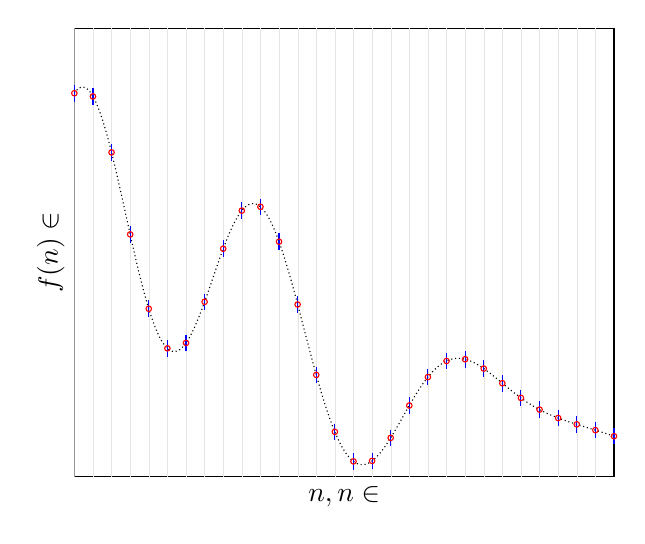
\begin{tikzpicture}
			\begin{axis} [
				xmin=\myxmin,xmax=\myxmax,
				ymin=\myymin,ymax=\myymax,
				xlabel={$n\sampletime, n \in \integers$},
				ylabel={$f(n\sampletime)  \in \realnumbers$},	
				xtick=\empty, 
				ytick=\empty, 
				]
				\foreach \i in {1, 2,...,\mynsamples}{
					\addplot[\mygridcolor, line width=0.1pt] coordinates {
						((\i-1)*\sampletimestep,\myymin) ((\i-1)*\sampletimestep,\myymax) 
					};
				}
				\addplot+[only marks, domain=\myxmin:\myxmax,samples=\mynsamples, mark color=\mycolor, mark=|, mark size=3pt, \mycolor]{\thefunction};
				\addplot+[only marks, domain=\myxmin:\myxmax,samples=\mynsamples, mark color=\mycolor, mark=o, mark size=1pt, mark options={fill=\mycolor, draw=\mycolor,}]{\thefunction};
				\addplot[domain=\myxmin:\myxmax,samples=1000, densely dotted, \mycolorii]{\thefunction};
			\end{axis}
		\end{tikzpicture}
	};	
	\node[anchor=center] (valdisc) at (0,-\myplotydist) {
		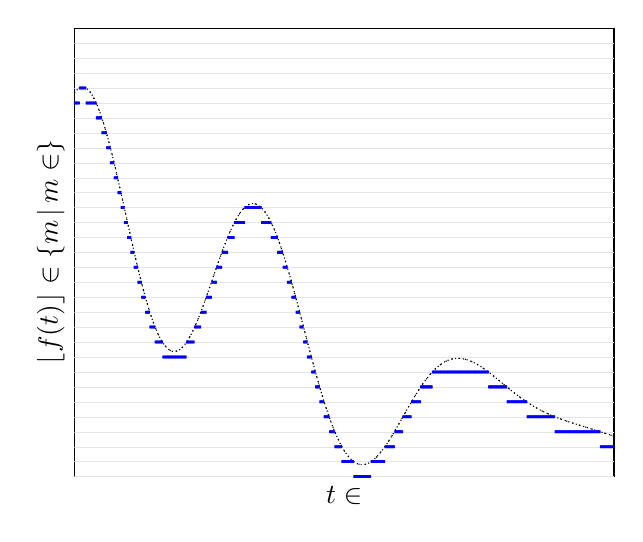
\begin{tikzpicture}
			\begin{axis} [
				xmin=\myxmin,xmax=\myxmax,
				ymin=\myymin,ymax=\myymax,
				xlabel= {$t  \in \realnumbers$},
				ylabel={$\lfloor f(t) \rfloor \in \{m\quantizestep \,\vert\, m \in \integers\}$},	
				xtick=\empty, 
				ytick=\empty, 
				]
				\foreach \i in {1, 2,...,\nquantsteps}{
					\addplot[\mygridcolor, line width=0.1pt] coordinates {
						(\myxmin, {(\i-1)*\quantizeres}) (\myxmax, {(\i-1)*\quantizeres}) 
					};
				}
				\addplot+[only marks,domain=\myxmin:\myxmax, samples=1001, \mycolor,mark=o,mark options={xscale=0.005, yscale=0.25}]{floor(\thefunction*\nquantsteps)/\nquantsteps};
				\addplot[domain=\myxmin:\myxmax,samples=1000, dotted, \mycolor]{\thefunction};
				\addplot[domain=\myxmin:\myxmax,samples=1000, densely dotted, \mycolorii]{\thefunction};
			\end{axis}
		\end{tikzpicture}
	};				
	\node[anchor=center] (timevaldisc) at (\myplotxdist,-\myplotydist) {
		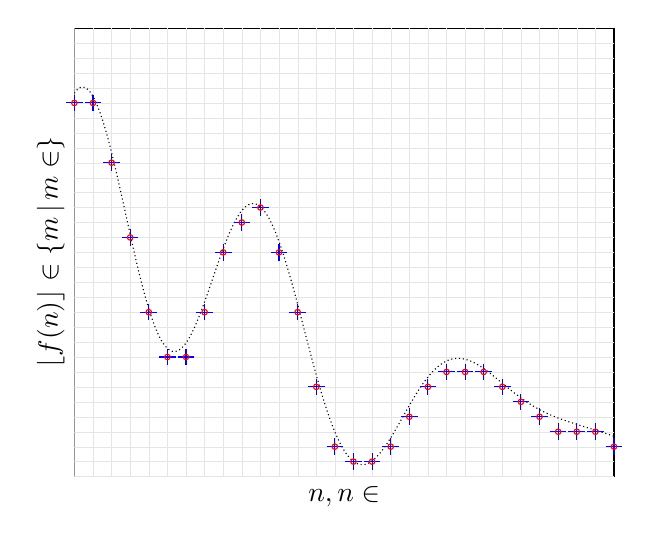
\begin{tikzpicture}
			\begin{axis} [
				xmin=\myxmin,xmax=\myxmax,
				ymin=\myymin,ymax=\myymax,
				xlabel= {$n\sampletime, n \in \integers$},
				ylabel={$\lfloor f(n\sampletime) \rfloor  \in \{m\quantizestep\,\vert\, m \in \integers\}$},	
				xtick=\empty, 
				ytick=\empty, 
				]
				\foreach \i in {1, 2,...,\nquantsteps}{
					\addplot[\mygridcolor, line width=0.1pt] coordinates {
						(\myxmin, {(\i-1)*\quantizeres}) (\myxmax, {(\i-1)*\quantizeres}) 
					};
				}
				\foreach \i in {1, 2,...,\mynsamples}{
					\addplot[\mygridcolor, line width=0.1pt] coordinates {
						((\i-1)*\sampletimestep,\myymin) ((\i-1)*\sampletimestep,\myymax) 
					};
				}
				\addplot+[only marks, domain=\myxmin:\myxmax,samples=\mynsamples, mark color=\mycolor, mark=+, mark size=3pt, \mycolor] {floor(\thefunction*\nquantsteps)/\nquantsteps};
				\addplot+[only marks, domain=\myxmin:\myxmax,samples=\mynsamples, mark color=\mycolor, mark=o, mark size=1pt, mark options={fill=\mycolor, draw=\mycolor,}]{floor(\thefunction*\nquantsteps)/\nquantsteps};
				\addplot[domain=\myxmin:\myxmax,samples=1000, densely dotted, \mycolorii]{\thefunction};
			\end{axis}
		\end{tikzpicture}
	};				
\end{tikzpicture}